\begin{figure}
\centering
    \begin{subfigure}{0.5\linewidth}
        
\includegraphics[width=\linewidth]{figures/accfluc/acc_fluc_legend.pdf}
    \end{subfigure}\\
    \begin{subfigure}{0.25\linewidth}
        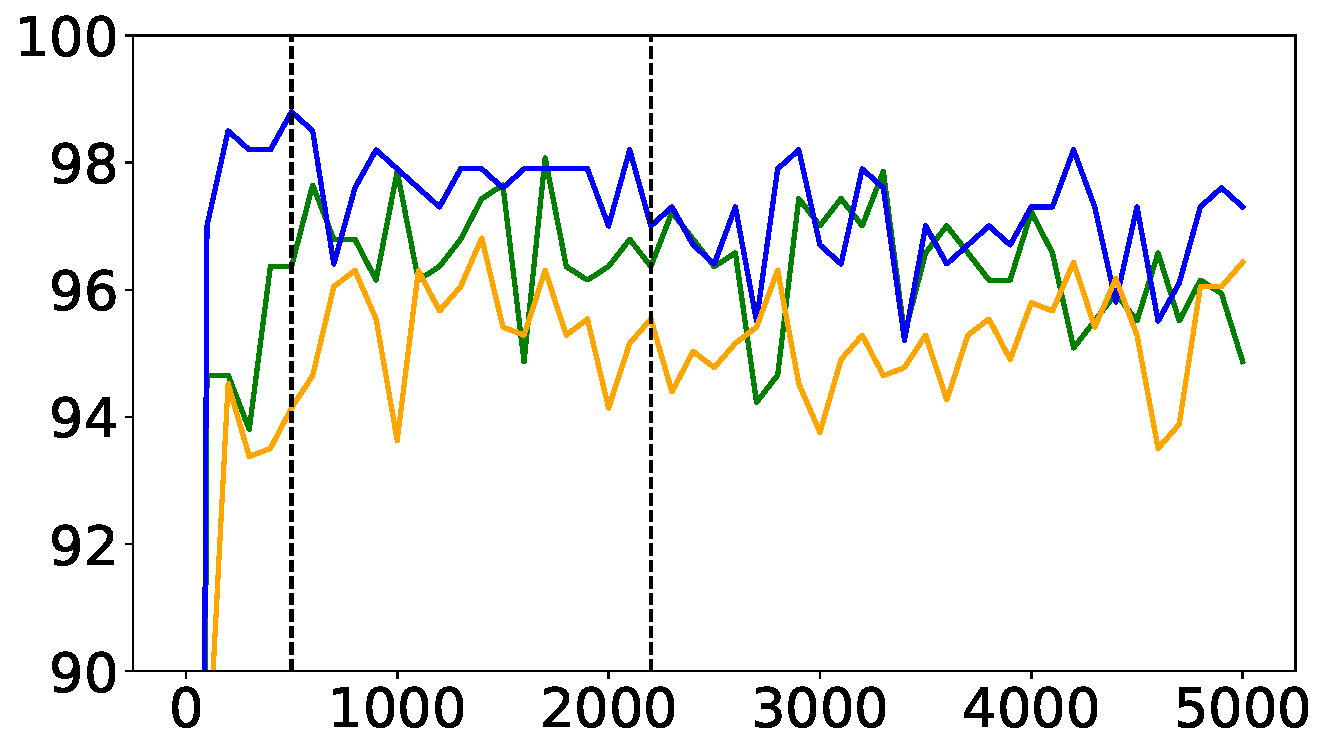
\includegraphics[width=\linewidth]{figures/accfluc/acc_fluc_TE0.pdf}%
        \caption{\small \textit{Art painting} (test)}
    \end{subfigure}%
    \begin{subfigure}{0.25\linewidth}
        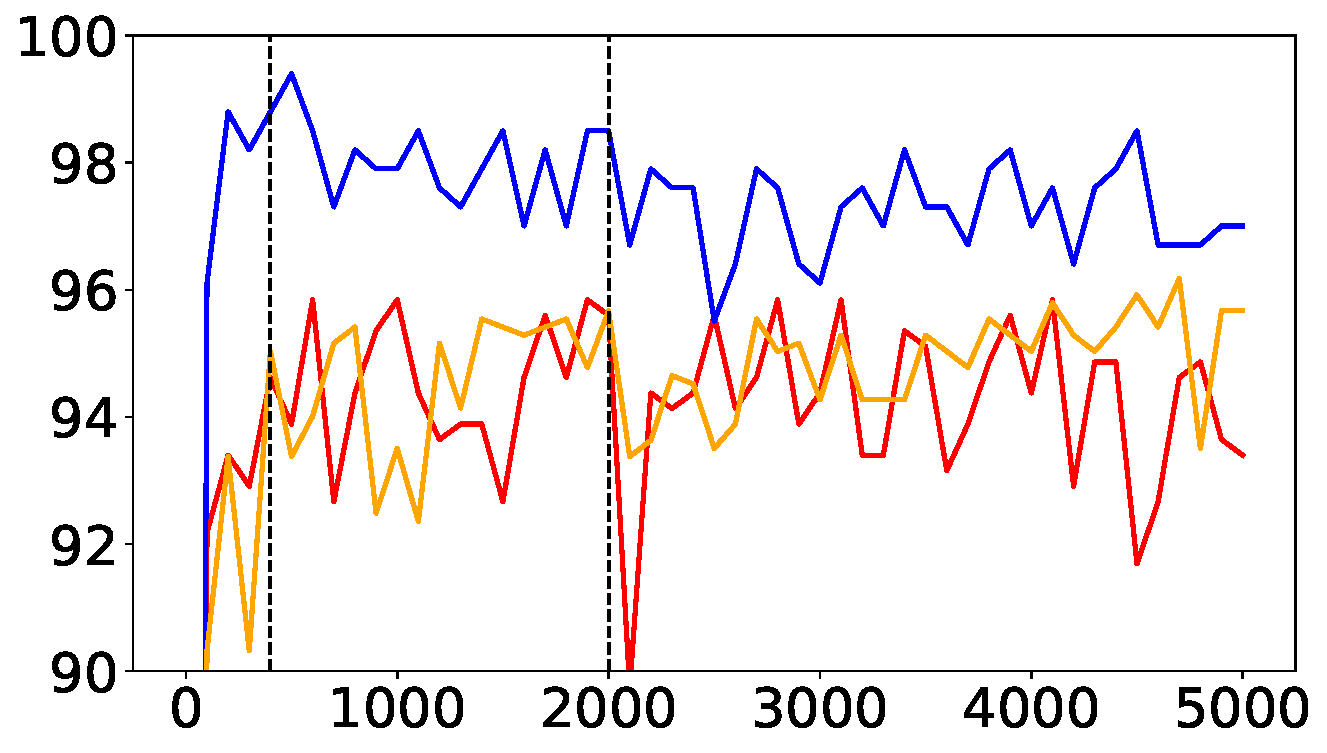
\includegraphics[width=\linewidth]{figures/accfluc/acc_fluc_TE1.pdf}%
        \caption{\small \textit{Cartoon} (test)}
    \end{subfigure}%
    \begin{subfigure}{0.25\linewidth}
        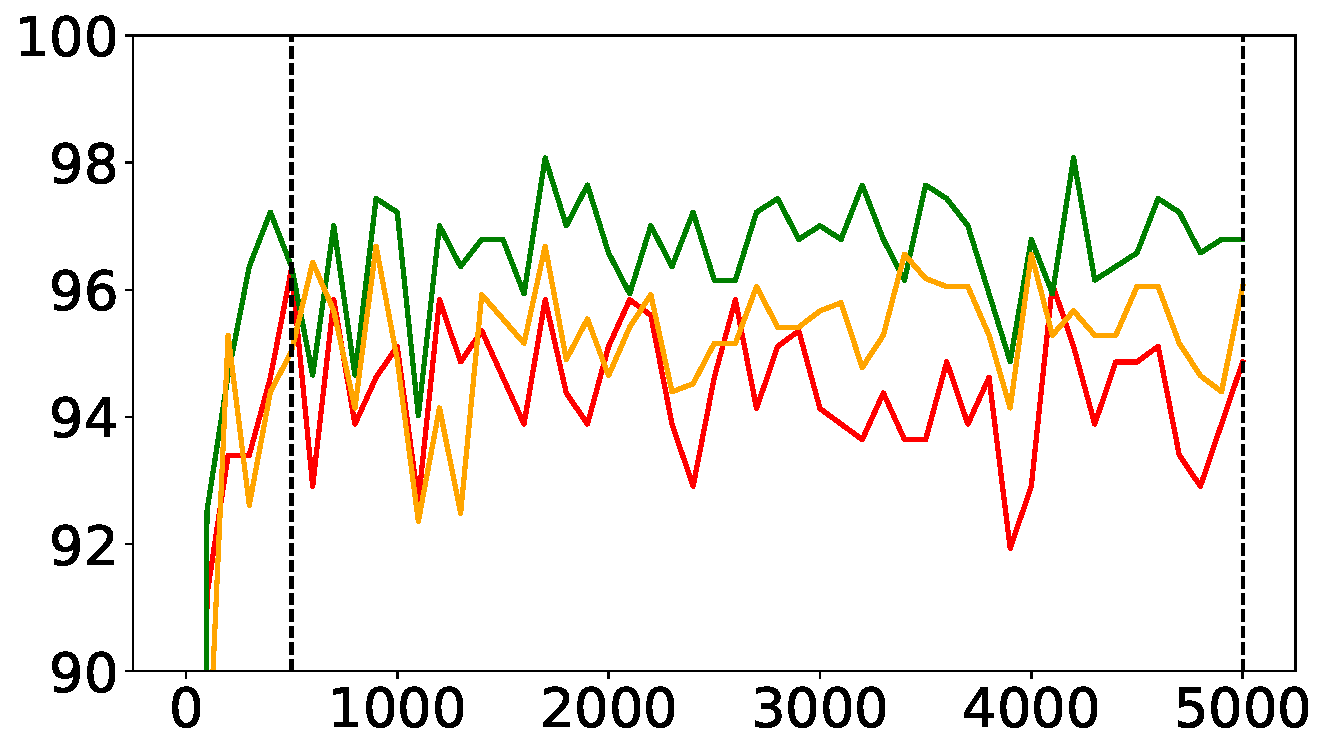
\includegraphics[width=\linewidth]{figures/accfluc/acc_fluc_TE2.pdf}%
        \caption{\small \textit{Photo} (test)}
    \end{subfigure}%
    \begin{subfigure}{0.25\linewidth}
        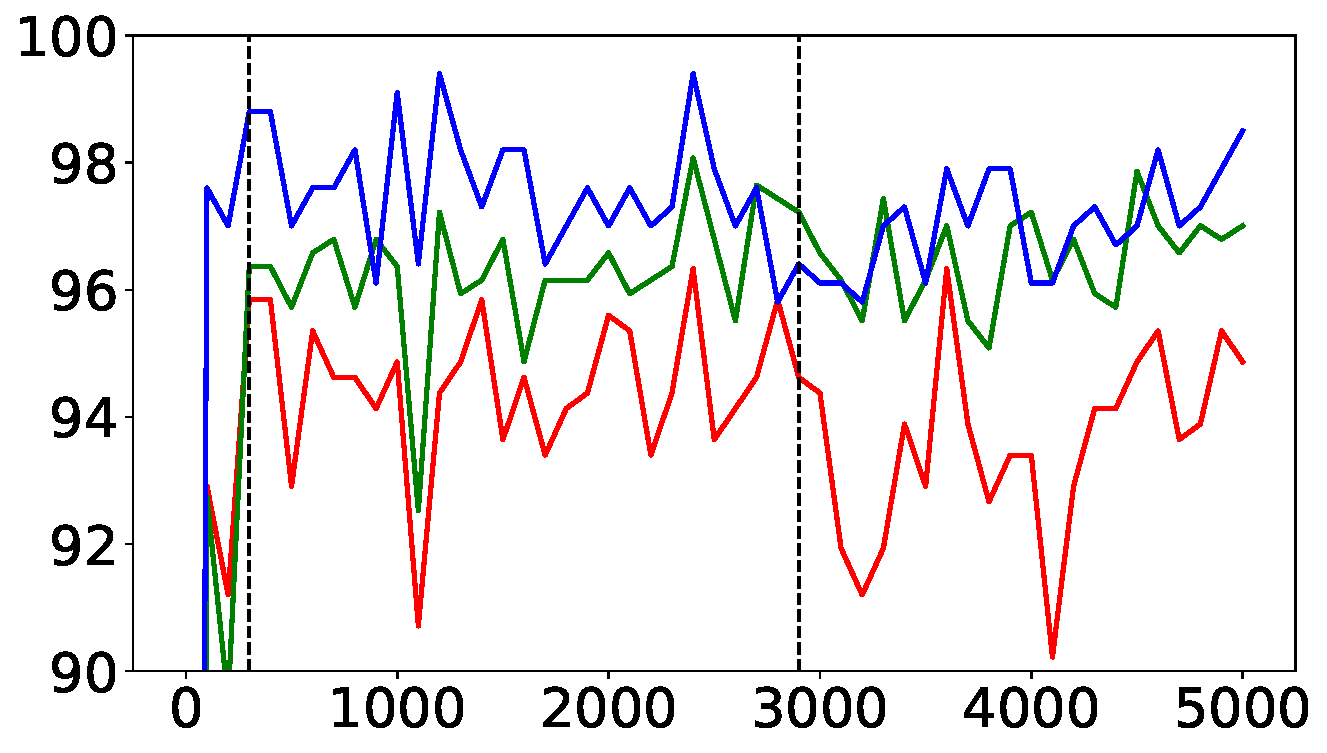
\includegraphics[width=\linewidth]{figures/accfluc/acc_fluc_TE3.pdf}%
        \caption{\small \textit{Sketch} (test)}
    \end{subfigure}%
    \caption{\small \textbf{Validation accuracies for in-domains.} The X- and Y-axis indicate the training iterations and accuracy, respectively, about the validation domains (legend) and the test domain (caption). The vertical dot lines represent start and end iterations, $t_s$ and $t_e$, identified by the overfit-aware sampling strategy of SWAD.}
    \label{fig:accfluc}
\end{figure}